% This is samplepaper.tex, a sample chapter demonstrating the
% LLNCS macro package for Springer Computer Science proceedings;
% Version 2.21 of 2022/01/12
%

\documentclass[runningheads]{llncs}
%
\usepackage[T1]{fontenc}
\usepackage{pdfpages}
\usepackage{tabularx}
\usepackage{booktabs}
\newcolumntype{Y}{>{\raggedright\arraybackslash}X}

% T1 fonts will be used to generate the final print and online PDFs,
% so please use T1 fonts in your manuscript whenever possible.
% Other font encondings may result in incorrect characters.
%
\usepackage{graphicx}
% Used for displaying a sample figure. If possible, figure files should
% be included in EPS format.
%
% If you use the hyperref package, please uncomment the following two lines
% to display URLs in blue roman font according to Springer's eBook style:
%\usepackage{color}
%\renewcommand\UrlFont{\color{blue}\rmfamily}
%\urlstyle{rm}
%
\begin{document}
%
\title{Knowledge Elicitation and Ontology-Based Visualization of Business Ecosystems: A Case Study from the 
Wind Energy Ecosystem}
%
%\titlerunning{Abbreviated paper title}
% If the paper title is too long for the running head, you can set
% an abbreviated paper title here
%
\author{Alican Tüzün\inst{1,2}\orcidID{0009-0009-8017-5487} \and
Georgios Meditskos\inst{1}\orcidID{0000-0003-4242-5245}
}
%
\authorrunning{Tüzün et al.}
% First names are abbreviated in the running head.
% If there are more than two authors, 'et al.' is used.
%
\institute{School of Informatics, Aristotle University of Thessaloniki, Thessaloniki, Greece\and
Josef Ressel Centre for Data-Driven Business Model Innovation, University of Applied Sciences Upper Austria, 
Wehrgrabengasse 1-4, 4400, Steyr, Austria
\email{lncs@springer.com}\\
\url{http://www.springer.com/gp/computer-science/lncs}}
%
\maketitle              % typeset the header of the contribution
%
\begin{abstract}
The abstract should briefly summarize the contents of the paper in
150--250 words.

\keywords{Business Ecosystem  \and Knowledge Representation \and Ontology \and Wind Energy \and Green Energy.}
\end{abstract}
%
%
%
\section{Introduction}




\subsection{P1: Hook}

\subsection{P2: Business, Wind Energy Ecosystems}

\subsection{P3:Ecosystem interactions}

\subsection{P4: Knowledge Representation, Ecosystem Knowledge}

\subsection{P5: Challange }

\subsection*{\textbf{Research Question}}
\begin{center}
    \textit{How can organizational interactions in the wind energy ecosystem 
systematically captured and explicitized into structured, formal knowledge representations to enable data-driven decision making?}
\end{center}

\section{Methology}

\subsection{Semi-Structured Survey}

\begin{table}[ht]
    \centering
    \caption{Relationships and Theoretical Foundations}
    \label{tab:relationships}
    \begin{tabularx}{\textwidth}{lYY}
    \toprule
    \textbf{Relationship Type} & \textbf{Theoretical Foundation} & \textbf{Logical Charecteristics} \\
    \midrule
    Product \& Service Delivery & 
    Supply Chain Management (Chopra \& Meindl, 2016); 
    Value Chain Analysis (Porter, 1985); 
    Business Ecosystems (Adner, 2017) & 
    Irreflexive, Transitive \\
    \addlinespace
    
    Payment & 
    Business Model Ontology (Osterwalder \& Pigneur, 2005); 
    Value Network Analysis (Allee, 2008); 
    Input-Output Economics (Leontief, 1986) & 
    Irreflexive \\
    \addlinespace
    
    Data & 
    Knowledge-Based View (Grant, 1996); 
    Digital Ecosystem Theory (Tiwana, 2013) &
    Irreflexive \\
    \addlinespace
    
    Information & 
    Knowledge-Based View (Grant, 1996) & 
    Irreflexive \\
    \addlinespace
    
    Collaboration & 
    Resource-Based View (Barney, 1991) & 
    Irreflexive, Symmetric \\
    \addlinespace
    
    Conflict & 
    Stakeholder Theory (Freeman, 1984) & 
    Irreflexive,ASymmetric \\
    \addlinespace
    
    Competition & 
    Porter's Five Forces (Porter, 1979) & 
    Irreflexive, Symmetric \\
    \addlinespace
    
    Coopetition (Implicit) & 
    Coopetition Theory (Brandenburger \& Nalebuff, 1996) & 
    Irreflexive \\
    \bottomrule
    \end{tabularx}
    \smallskip
    \end{table}

\subsection{Term Disambiguation}

\subsection{OWL2 \& Ontological Commitments}

\begin{itemize}
    \item \textbf{ClassAssertion}
    \item \textbf{ClassHierarchyAssertion}
    \item \textbf{ClassDisjointnessAssertion}
    \item \textbf{ObjectPropertyAssertion}
    \item \textbf{PropertyCharacteristicAssertions}
    \item \textbf{Methodological Limitations}
\end{itemize}

\subsection{Query Language}
\begin{itemize}
    \item \textbf{SPARQL}
    \item \textbf{Fuseki Server}
\end{itemize}
\subsection{Relationship Visualization}
\begin{itemize}
    \item \textbf{js and d3.js}
\end{itemize}

\section{Results\&Discussion}

\subsection{Survey Results\&Discussion}

\subsection{Ontology Development}
\subsection{Information Retrieval with Sparql}
\subsection{Visualization Results}

\section{Conclusion}

\section{Appendix}
\appendix
\section{Semi-Structured Survey}
%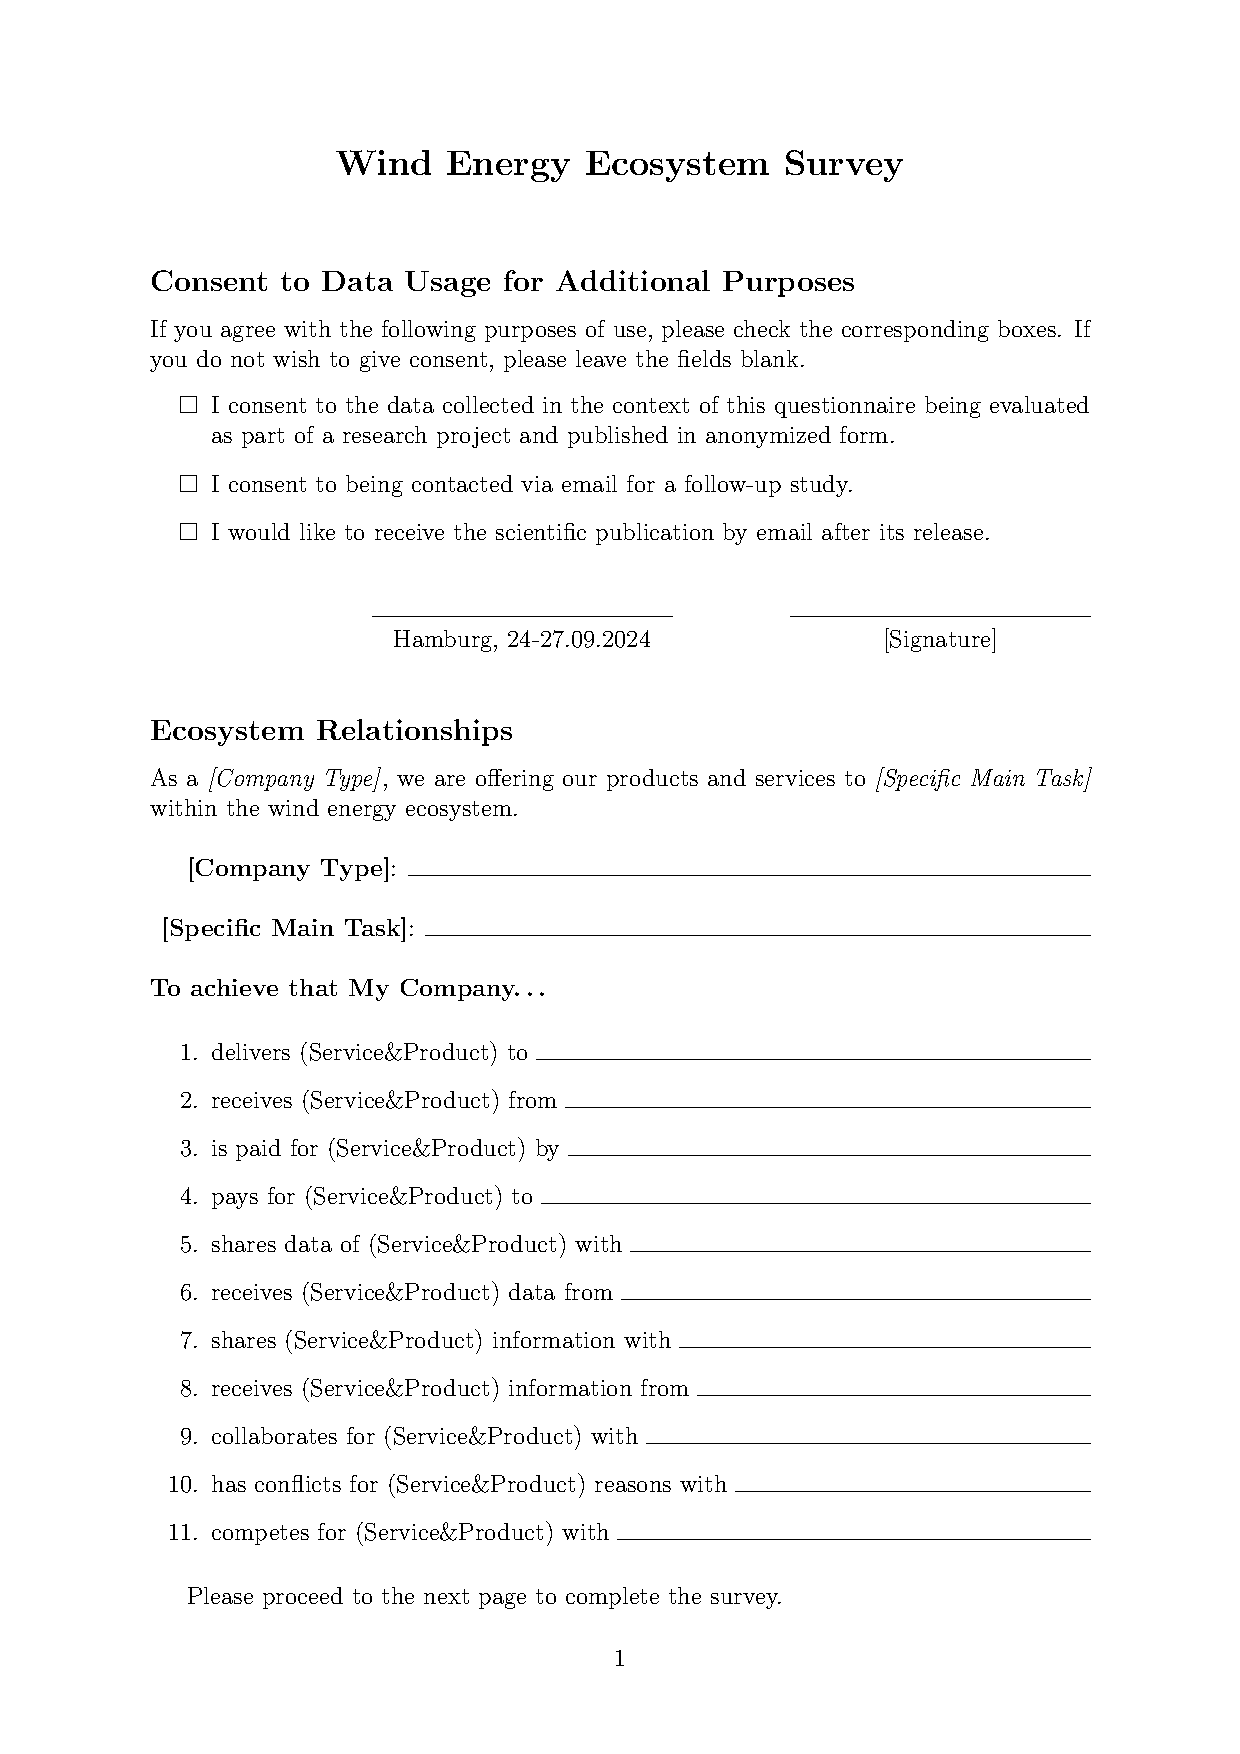
\includepdf[pages=-]{survey.pdf}
\section{Github Repo}

\bibliographystyle{splncs04}
\bibliography{reference}

Main idea: Conventional modeling approaches does not leverage semantics, therefore the visualizations gets too complex such that decision makers cannot comprehend.
However with the SPARQL querries, one can easily semantically query the information (e.g traversing the graphs) and visualize whatever needed for the decision maker. With the former 
methodologies it is not possible.

Sub effect: Because of the formality, one can also use the symbolic logic therefore can infer new relationships within the data, which is also not possible with the conventional methods.


Sub effect: Formal and needed representations reduces the ambiguity and the complexity of the data, therefore the decision makers can easily understand the data and make decisions.

Analogy: To go through something with a fine-tooth comb 

\end{document}

